\documentclass[12pt,a4paper]{article}
\usepackage[a4paper,margin=1in]{geometry}
\usepackage{hyperref}
\usepackage{titlesec}
\usepackage{enumitem}
\usepackage{setspace}
\usepackage{lmodern}
\usepackage[T1]{fontenc}
\usepackage{fancyhdr}
\usepackage{titlesec}
\usepackage{graphicx}


\setstretch{1.2}

\setlength{\parindent}{0pt}
\setlength{\parskip}{1em}

\titleformat{\section}{\Large\bfseries}{\thesection}{1em}{}
\titleformat{\subsection}{\large\bfseries}{\thesubsection}{1em}{}
\titleformat{\subsubsection}{\normalsize\bfseries}{\thesubsubsection}{1em}{}
\titleformat{\paragraph}[block]{\normalsize\bfseries}{\theparagraph}{1em}{}
\titlespacing*{\paragraph}{0pt}{1em}{0.5em}
\titleformat{\subparagraph}[block]{\normalsize\bfseries}{\thesubparagraph}{1em}{}
\titlespacing*{\subparagraph}{0pt}{1em}{0.5em}


\title{\textbf{Local Multimodel Assistant for Visual Studio Code}}
\date{}

\pagestyle{fancy}
\fancyhf{}
\pagenumbering{gobble}

\begin{document}

\begin{titlepage}
    \centering
    BABE\c S BOLYAI UNIVERSITY, CLUJ NAPOCA, ROM\^ ANIA
    FACULTY OF MATHEMATICS AND COMPUTER SCIENCE
    \vspace*{4cm}

    {\Huge\textbf{Multimodel VS Code Extension}}\\[2cm]

    \vspace{5cm}

    \begin{flushright}
        {\Large\textbf{Team Members}}\\[1cm]
        \textbf{Croitoru Andreea-Bianca} \\ Group 232 \\[0.3cm]
        \textbf{Dobrescu Paul Andrei} \\ Group 232 \\[0.3cm]
        \textbf{Moghioros Eric} \\ Group 234
    \end{flushright}

    \vspace*{3cm}
    2025-2026

\end{titlepage}

\newpage
\tableofcontents

\setstretch{1.5}

\newpage
\pagenumbering{arabic}
\pagestyle{plain}

\maketitle

\section{Introduction}

\subsection{Context}

The Multimodel AI Assistant project aims to develop an extension for the Visual Studio Code environment that integrates 
advanced intelligent assistance functionalities into the software development process. The main objective is to create a 
tool capable of supporting developers in activities such as code analysis and review, security vulnerability detection, 
project knowledge management, and workflow optimization through the orchestration of multiple artificial intelligence 
models.

The proposed system employs a multimodal architecture, in which several AI models, both local and cloud-based, 
collaborate to generate contextual and efficient responses. This approach enables dynamic adaptation of computational 
resources, performance optimization, and data confidentiality, depending on the specific characteristics of the analyzed 
project.

\subsection{Motivation}

In the current context of software development, the complexity of information systems has increased significantly, 
generating a growing need for tools that facilitate the automation of analysis and verification processes. Modern 
software projects involve thousands of lines of code, geographically distributed teams, and strict quality and security 
requirements. Under these circumstances, traditional manual code review methods become inefficient and error-prone to 
humans.

The motivation for employing an intelligent algorithm within this project arises from the necessity of optimizing the 
development process through the following aspects:

\begin{itemize}[leftmargin=1.5em]
    \item \textit{Operational efficiency:} AI systems can automatically analyze extensive code segments, rapidly 
    identifying errors, inconsistencies, or potential vulnerabilities.
    \item \textit{Continuous and adaptive learning:} The system can accumulate knowledge from previous projects, 
    adapting to the team’s coding style and the specific domain of the application.
    \item \textit{Enhanced software security:} Automated analysis modules can identify vulnerabilities that are 
    difficult to detect through conventional methods, thus reducing security risks.
    \item \textit{Data confidentiality:} Through support for local models, code analysis can be performed internally 
    without exposing sensitive information to external services.
\end{itemize}

Therefore, the implementation of a solution based on intelligent algorithms represents an essential step toward 
modernizing the software development process, ensuring a balance between performance, security, and adaptability.

\section{Contemporary Holdbacks}

Artificial intelligence has emerged as a promising approach for automating parts of the software development process. 
Large language models (LLMs) and machine learning systems can analyze source code, generate documentation, and provide 
intelligent suggestions. However, current AI-powered tools often suffer from three critical limitations:

\begin{itemize}[leftmargin=1.5em]
    \item \textit{Single-model dependency:} Most tools rely on one large, centralized model, which limits flexibility 
    and adaptability across diverse tasks.
    \item \textit{Privacy and security concerns:} Cloud-based AI services require sending source code to external 
    servers, raising confidentiality and compliance issues for organizations handling sensitive or proprietary data.
    \item \textit{Lack of contextual learning:} Existing systems typically provide isolated, one-time analyses without 
    learning from past interactions or adapting to the specific coding practices of a development team.
\end{itemize}

The scientific contribution lies in developing a framework that merges AI orchestration, knowledge-based adaptation, and 
privacy-aware computation into a unified assistant. This framework represents a new step toward intelligent software 
development environments, where artificial intelligence operates not as a single tool but as a coordinated ecosystem of 
models that understand, learn, and evolve with the developer’s workflow.

\section{Related Work}

The development of intelligent software assistants has received increasing attention in recent years, driven by advances 
in natural language processing, machine learning, and software engineering tools. Several approaches have been proposed 
to support developers in tasks such as code review, vulnerability detection, documentation generation, and automated 
refactoring.

\subsection{\href{https://github.com/openai/codex}{OpenAI Codex}}

\begin{itemize}[leftmargin=1.5em]
    \item \textit{Data:} The original OpenAI Codex model was trained on approximately 159 GB of Python code from over 54 
    million public GitHub repositories, covering multiple programming languages including JavaScript, Go, Ruby, and C++. 
    The dataset included a range of software projects from simple scripts to complex applications, curated to ensure 
    high quality and adherence to good programming practices. Reinforcement learning from human feedback (RLHF) was 
    incorporated in later versions to improve autonomous coding capabilities and understand real-world coding scenarios.
    \item \textit{Algorithm:} Codex is based on the GPT-3 architecture fine-tuned specifically for programming tasks. It 
    operates by analyzing input prompts—such as natural language descriptions or partial code snippets—and predicting 
    the most probable continuation of code tokens. The model uses statistical patterns learned from the training data to 
    generate code but does not execute or logically reason about the code. Iterative prompt refinement helps improve the 
    quality of generated code.
    \item \textit{Outcomes:} Codex can complete approximately 37\% of coding requests accurately and generates working 
    solutions for around 70\% of test prompts when sampled multiple times. It supports over a dozen programming 
    languages with highest performance in Python. Codex accelerates programming by generating code snippets, automating 
    tasks like opening pull requests, refactoring files, and writing tests. Its limitations include occasional errors 
    and dependence on prompt quality, making it a tool to assist rather than replace human developers.
\end{itemize}

\subsection{\href{https://arxiv.org/abs/2505.16339}{Rethinking Code Review Workflows with LLM Assistance}}

\begin{itemize}[leftmargin=1.5em]
    \item \textit{Data:} The study used empirical data from an industrial field study conducted at WirelessCar Sweden 
    AB, comprising semi-structured interviews and real-world experiments with two prototype LLM-assisted code review 
    tools. The tools integrated retrieval-augmented generation (RAG) to provide contextual information during code 
    reviews, addressing challenges like frequent context switching and insufficient context.
    \item \textit{Algorithm:} Two variations of LLM-assisted review tools were developed: one providing upfront 
    LLM-generated reviews (AI-led co-reviewer) and another offering on-demand interaction with the LLM (interactive 
    assistant). Both leveraged semantic search pipelines to retrieve relevant information and augment reviews with 
    context for increased accuracy and developer support.
    \item \textit{Outcomes:} The field experiment demonstrated that AI-led, upfront reviews were generally preferred by 
    developers, although acceptance depended on the reviewer’s familiarity with codebases and pull request severity. Key 
    benefits included reduced context switching and improved review efficiency, though concerns about false positives 
    and trust in the AI were noted. The approach showed promise for enhanced developer experience and workflow 
    optimization.
\end{itemize}

\subsection{\href{https://arxiv.org/abs/2510.01379}{Enhanced Code Generation via Multi-Stage Performance-Guided LLM 
Orchestration}}

\begin{itemize}[leftmargin=1.5em]
    \item \textit{Data:} This work conducted a comprehensive empirical study analyzing the performance of 17 
    state-of-the-art LLMs on the HumanEval-X benchmark across five programming languages (Python, Java, C++, Go, Rust). 
    The dataset included various algorithmic domains and development stages, evaluated with functional correctness and 
    runtime metrics such as execution time and memory usage.
    \item \textit{Algorithm:} The authors introduced PerfOrch, a multi-stage LLM orchestration framework that 
    dynamically routes code generation tasks to the most suitable LLMs following a generate-fix-refine workflow. It 
    incorporates stage-wise validation and rollback mechanisms without requiring model fine-tuning. The system uses 
    performance guidance based on empirical profiling to select LLMs for each task context.
    \item \textit{Outcomes:} PerfOrch outperformed single-model baselines with correctness rates of 96.22\% on 
    HumanEval-X and 91.37\% on EffiBench-X, surpassing GPT-4o’s 78.66\% and 49.11\%. Additionally, it improved execution 
    speeds for over half of the tested problems with median speedups of 17.67\% to 27.66\%, demonstrating both 
    correctness and efficiency improvements. The framework’s scalability and plug-and-play design allow continual 
    integration of new models.
\end{itemize}

\subsection{\href{https://arxiv.org/abs/2504.08525}{Enhancing State Awareness for Multi-Step LLM Agent Tasks}}

\begin{itemize}[leftmargin=1.5em]
    \item \textit{Data:} The proposed Task Memory Engine (TME) was evaluated through case studies and comparative 
    experiments on multi-step agent tasks, with datasets involving hierarchical task structures and sub-task 
    relationships to test multi-step reasoning and execution consistency.
    \item \textit{Algorithm:} TME is a lightweight, structured memory module that employs a hierarchical Task Memory 
    Tree (TMT). Each node corresponds to a task step and stores input, output, status, and sub-task relationships. A 
    prompt synthesis method dynamically generates LLM prompts based on the active node path to maintain contextual 
    grounding and improve task execution coherence over multiple steps.
    \item \textit{Outcomes:} TME led to better task completion accuracy, more interpretable agent behavior, and reduced 
    hallucinations in multi-step LLM applications with minimal implementation overhead. The structured memory improved 
    long-range coherence and robustness of autonomous LLM agents in executing complex, multi-step tasks.
\end{itemize}

This summary provides an overview of the data sources, core algorithms, and key results from these recent works on 
intelligent software assistants and LLM-based programming support systems.

\section{Multi-Agent System Architecture}

This section presents the design, responsibilities, and coordination logic of the multi-agent orchestration framework implemented in the system. The architecture adopts a distributed model in which four specialized agents --- the \textit{Main Agent}, \textit{Architecture Agent}, \textit{Builder Agent}, and \textit{Review Agent} --- collaborate to process user requests, generate code, validate software architecture, and perform quality assurance tasks. Each component operates under strict behavioral and communication constraints, enabling a reliable and deterministic pipeline.

The agents communicate exclusively through structured JSON messages, ensuring unambiguous, machine-readable interactions suitable for automated pipelines or scalable multi-model execution.

\subsection{Agent Overview}
\subsubsection{Main Agent}

The Main Agent serves as the orchestrator and central decision-making component of the system. It is the only agent permitted to communicate with the user directly. Its responsibilities include:

\begin{itemize}
    \item Interpreting the user's intent and request semantics.
    \item Determining whether the request requires the full multi-agent development pipeline (Flow~1) or a direct non-code response (Flow~2).
    \item Delegating tasks to the Architecture, Builder, or Review agents when appropriate.
    \item Managing workflow ordering, context propagation, and JSON message formatting.
    \item Ensuring that architectural design, code generation, and review steps occur in the correct sequence.
\end{itemize}

The Main Agent does \textbf{not} generate, evaluate, or modify code. Instead, it acts as a controller that routes tasks to more specialized agents. It ensures that architectural validation precedes code generation and that code is always reviewed before being communicated back to the user.

\paragraph{Communication Behavior}
The Main Agent produces three types of JSON messages:

\begin{enumerate}
    \item \textbf{Delegation Messages} sent to Architecture, Builder, or Review agents.
    \item \textbf{User Responses} when the output is final or when Flow~2 is selected.
    \item \textbf{File Requests} when additional project files are required to continue the workflow.
\end{enumerate}

\subsubsection{Architecture Agent}

The Architecture Agent is responsible for evaluating and refactoring code from a structural and architectural perspective. Its role focuses on high-level software engineering principles, including modularity, maintainability, design patterns, and adherence to SOLID principles.

Key responsibilities include:

\begin{itemize}
    \item Detecting architectural anti-patterns such as cyclic dependencies, tight coupling, or god classes.
    \item Enforcing separation of concerns, clean boundaries, and correct layering.
    \item Correcting or refining class design, dependency direction, and module organization.
    \item Refactoring code when structural improvements are necessary, while preserving functionality.
\end{itemize}

The Architecture Agent outputs:

\begin{itemize}
    \item A full corrected file (never partial or diff-based).
    \item A detailed list of architectural fixes.
    \item A summary of the refactoring performed.
    \item A routing directive (\texttt{"next\_node"}) indicating whether execution should proceed to the Builder Agent.
\end{itemize}

\paragraph{Communication Behavior}
The Architecture Agent sends a JSON message back to the Main Agent, which then forwards the output to the Builder Agent for implementation of structural changes in new or existing files.

\subsubsection{Builder Agent}

The Builder Agent is the code implementation model responsible for generating and modifying program files based on instructions received from the Architecture Agent. It is a deterministic code generator with the following capabilities:

\begin{itemize}
    \item Creating new files when specified.
    \item Modifying existing files while preserving required functionality.
    \item Applying reviewer feedback precisely and without deviation.
    \item Producing complete file content for all modified components.
\end{itemize}

The Builder Agent outputs a structured JSON object that includes:

\begin{itemize}
    \item Fully generated or modified files.
    \item Optional dependencies introduced by the new implementation.
    \item Setup instructions when required.
    \item A task list for the Review Agent.
\end{itemize}

\paragraph{Communication Behavior}
The Builder Agent always forwards its output to the Review Agent. No direct communication with the user or the Architecture Agent occurs.

\subsubsection{Review Agent}

The Review Agent functions as a readability and style correctness evaluator. It ensures that the generated code adheres to standard software quality guidelines related to:

\begin{itemize}
    \item Readability, naming clarity, and consistent formatting.
    \item Removal of dead, redundant, or confusing code.
    \item Simplification of expressions or refactoring long methods.
    \item Ensuring code follows human-centered readability principles.
\end{itemize}

The Review Agent acts like a linter and applies only non-functional improvements. It must return:

\begin{itemize}
    \item A full, corrected version of the file.
    \item A list of readability and style improvements.
    \item A short summary of applied changes.
    \item A \texttt{"next\_node"} directive, which is always set to \texttt{"none"}.
\end{itemize}

\subsection{Inter-Agent Communication Protocol}

Communication between agents is strictly governed by JSON schemas. Outputs from one agent act as inputs for the next, ensuring deterministic workflows. The communication takes place exclusively in the following direction:

\begin{center}
\textbf{Main} $\rightarrow$ \textbf{Architecture} $\rightarrow$ \textbf{Builder} $\rightarrow$ \textbf{Review} $\rightarrow$ \textbf{Main}
\end{center}

Each agent returns structured outputs that must be:

\begin{itemize}
    \item Valid JSON.
    \item Complete and self-contained.
    \item Suitable for direct machine parsing.
    \item Free of commentary, markdown, or partial information.
\end{itemize}

\subsection{Workflow Models}

\begin{figure}[h!]
    \centering
    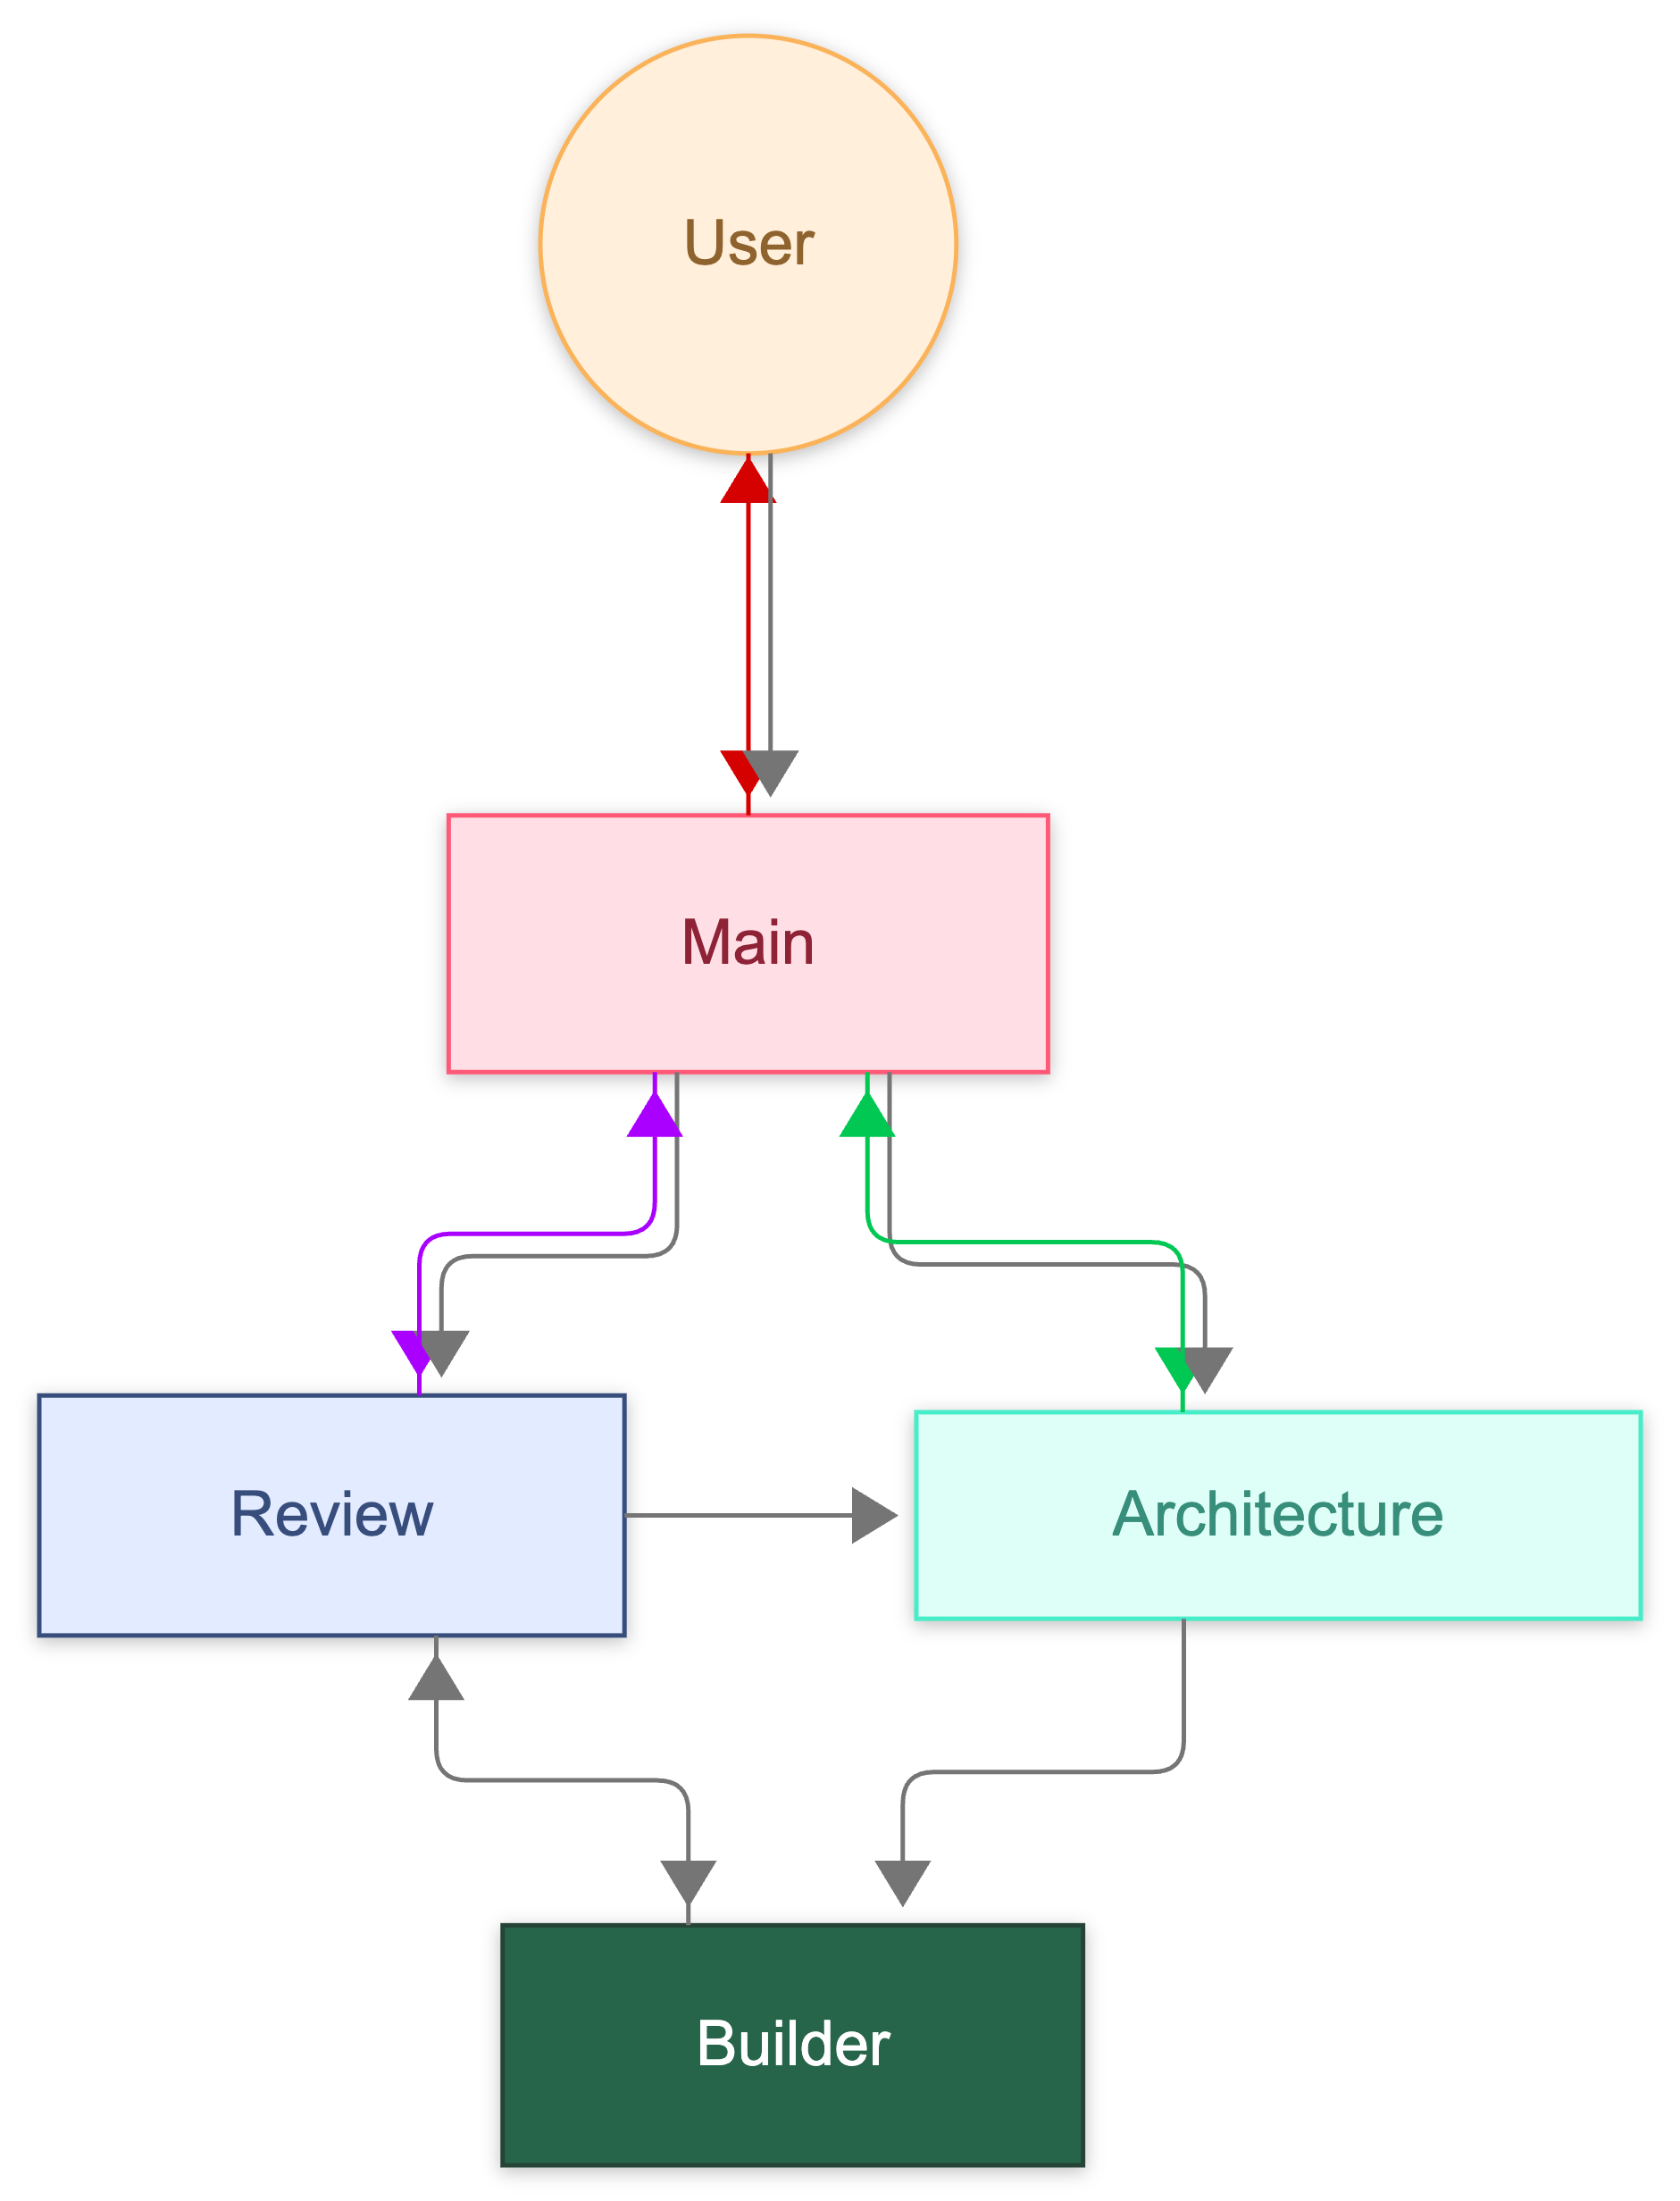
\includegraphics[width=0.7\textwidth]{assets/MA_diagram.png}
    \caption{Workflow diagram}
    \label{fig:workflow}
\end{figure}

\subsubsection{Flow 1: Full Development Pipeline}

Flow~1 is executed when the user's request requires architectural reasoning, code generation, modification, extension, debugging, or any form of code analysis. This workflow consists of the following stages:

\begin{enumerate}
    \item \textbf{User Request} reaches the Main Agent.
    \item The Main Agent determines that architectural or code tasks are required.
    \item The request is delegated to the Architecture Agent for structural analysis.
    \item The Architecture Agent refactors the file and forwards its output to the Builder Agent.
    \item The Builder Agent generates code and sends it to the Review Agent.
    \item A loop may occur:
    \[
    \textbf{Builder} \leftrightarrow \textbf{Review}
    \]
    until the Review Agent is satisfied.
    \item The Main Agent validates pipeline completion and responds to the user.
\end{enumerate}

\subsubsection{Flow 2: Direct Response Pipeline}

Flow~2 applies to requests that require conceptual explanations, documentation, or non-programming answers. The workflow is:

\[
\textbf{User} \rightarrow \textbf{Main Agent} \rightarrow \textbf{User}
\]

No delegation to other agents occurs.

\subsubsection{Flow 3: Direct Review Pipeline}

Flow 3 is triggered when the user provides existing code and specifically requests a review for style, readability, or minor optimizations without requiring new feature implementation or architectural restructuring. In this scenario, the Main Agent bypasses the Architecture and Builder agents to engage the Review Agent directly.

\[
\textbf{User} \rightarrow \textbf{Main Agent} \rightarrow \textbf{Reviewer} \rightarrow \textbf{Main Agent} \rightarrow \textbf{User} 
\]

\begin{itemize} \item \textbf{Trigger:} The user submits code with a prompt such as "Review this for readability" or "Clean up this function". \item \textbf{Delegation:} The Main Agent identifies that no structural changes are needed and routes the code directly to the \textbf{Review Agent}. \item \textbf{Outcome:} The Review Agent applies non-functional improvements and returns the refined code to the Main Agent, which then presents it to the user. \end{itemize}

\subsubsection{Flow 4: Direct Architectural Consultation}

Flow 4 is utilized when a user seeks high-level design advice, structural planning, or a critique of an existing project's organization without requesting immediate code generation. This flow optimizes token usage by avoiding the implementation and review stages when only conceptual guidance is required.

\[
\textbf{User} \rightarrow \textbf{Main Agent} \rightarrow \textbf{Architecture Agent} \rightarrow \textbf{Main Agent} \rightarrow \textbf{User} 
\]

\begin{itemize} \item \textbf{Trigger:} The user asks questions regarding design patterns, project structure, or SOLID principles, such as "How should I structure a Django app for this feature?". \item \textbf{Delegation:} The Main Agent delegates the request exclusively to the \textbf{Architecture Agent}. \item \textbf{Outcome:} The Architecture Agent provides an architectural summary or a refactoring plan without forwarding tasks to the Builder Agent. The Main Agent then communicates these high-level recommendations back to the user. \end{itemize}

\subsection{System Behavior and Determinism}

The system is designed to be deterministic and reproducible. Core behavioral rules include:

\begin{itemize}
    \item Agents must never perform tasks outside their specialization (e.g., Main Agent writing code).
    \item No agent may produce incomplete outputs.
    \item All file outputs must be complete and rewritten in full.
    \item Code must always be reviewed before being presented to the user.
    \item The Main Agent must select the correct workflow based on intent detection.
\end{itemize}

\subsection{Conclusion}

The multi-agent architecture provides a modular, reliable, and robust pipeline for generating high-quality software. Each agent specializes in a well-defined aspect of the software engineering lifecycle, and through strict communication protocols, the system ensures architectural correctness, production-quality code, and human-readable output. The specialization and cooperation of all four agents allow the system to scale to complex tasks while maintaining clarity, determinism, and correctness.

\section{Investigated Approaches for Compliance Checking Agent}
\subsection{Document Upload}

\subsubsection{Data Indexing and Chunking}

\paragraph{Importance of Chunking}
Chunking constitutes a central preprocessing operation in Retrieval-Augmented Generation (RAG) pipelines. Its primary purpose is to partition long documents into smaller, semantically coherent segments that can be efficiently embedded, stored, retrieved, and interpreted by downstream language models. Chunking directly addresses several constraints of modern LLM-based architectures:

\begin{itemize}
    \item \textbf{Token Limit Constraints:} Large documents frequently exceed the context windows of modern LLMs. Chunking mitigates this issue by enabling processing in smaller, context-preserving units.
    \item \textbf{Retrieval Accuracy:} Retrieval models (e.g., dense vector search, cosine similarity) perform significantly better when the indexed units contain a single, focused concept rather than multi-topic content.
    \item \textbf{Context Preservation:} Maintaining local semantic coherence ensures that retrieved chunks provide relevant and meaningful information during generation.
    \item \textbf{Computational Efficiency:} Smaller, well-defined chunks reduce embedding computation time and memory consumption.
    \item \textbf{Flexibility Across Document Types:} Technical documents, policies, rule sets, and legal texts vary in structure; chunking must adapt accordingly.
\end{itemize}

Overall, chunking plays the role of an intermediary layer that bridges data retrieval and generative reasoning, ensuring accurate, traceable, and contextually grounded results. Without an adequate chunking strategy, RAG-based systems tend to hallucinate, lose context, or return irrelevant results.

\paragraph{Types of Chunking}

\subparagraph{Fixed-Size Chunking}
A method in which the text is divided into uniform units based on a predefined token, word, or character count.

\textbf{Advantages:} Simple to implement, scalable, predictable behavior.\\  
\textbf{Disadvantages:} High risk of semantic fragmentation; unrelated information may accidentally be merged, thereby harming retrieval relevance.

\subparagraph{Sentence-Based Chunking}
The document is split according to natural sentence boundaries, optionally grouping consecutive sentences.

\textbf{Advantages:} Preserves grammatical and semantic flow; improves relevance of retrieved chunks.\\  
\textbf{Disadvantages:} Chunk sizes vary significantly; additional logic is required for grouping sentences.

\subparagraph{Semantic-Based Chunking}
The text is segmented based on semantic similarity or topic coherence, typically using cosine similarity between sentence embeddings.

\textbf{Advantages:} Strongest preservation of semantic boundaries; high-quality retrieval performance; adaptable to heterogeneous document structures.\\  
\textbf{Disadvantages:} Computationally more expensive; requires embedding inference during chunking.

\subparagraph{Document-Specific Chunking}
Chunking logic is adapted to the document’s intrinsic structure (e.g., headings, numbered lists, articles, subclauses, or tables).

\textbf{Advantages:} Excellent contextual fidelity; ideal for legal, policy, and regulatory documents.\\  
\textbf{Disadvantages:} Complex preprocessing requirements; dependent on accurate structure detection.

\subparagraph{Agentic Chunking}
Chunking designed around the operational tasks that an AI agent must perform (e.g., classification, retrieval, compliance checking).

\textbf{Advantages:} Task-specific optimization, enhanced interpretability, suitable for multi-agent frameworks.\\  
\textbf{Disadvantages:} Requires additional modeling and task understanding; harder to generalize.

\subsubsection{Embedding}
Embeddings encode text into high-dimensional vector representations that preserve semantic relationships. These vector representations are fundamental for similarity search, contextual retrieval, clustering, and semantic indexing.

\subsubsection*{Types of Embedding Models}

\paragraph{Word-Level Models}
Examples: Word2Vec, GloVe, FastText.\\  
Assign fixed vectors to words irrespective of context, useful for simple tasks, limited for nuanced semantic interpretation.

\paragraph{Contextual Embedding Models}
Examples: BERT, RoBERTa, sentence-transformers.\\ 
Embeddings vary according to surrounding context, enabling deeper semantic understanding.

\paragraph{Sentence and Document Embedding Models}
Examples: Sentence-BERT, E5, OpenAI embeddings.\\
Generate embeddings for entire sentences or paragraphs, making them highly suitable for retrieval tasks involving long-form documents.

\subsection{Token Efficiency and Data Representation}

Efficient management of context windows and token consumption is a critical constraint in Large Language Model (LLM) applications. This system incorporates specific strategies to monitor usage and optimize data serialization.

\subsubsection{Token Counting Mechanism}

To maintain operational visibility and manage costs associated with LLM inference, the system implements a granular token tracking mechanism.

\begin{itemize}[leftmargin=1.5em]
    \item \textbf{Data Persistence:} The schema for the \texttt{Message} model has been extended to include a \texttt{tokens\_used} field. This allows for the storage of precise consumption metrics for every interaction within a conversation thread.
    \item \textbf{Usage Extraction:} The \texttt{ModelManager} service parses the standardized \texttt{usage} payload returned by the inference API (e.g., OpenRouter or OpenAI). It extracts the \texttt{total\_tokens} count immediately after generation and persists it alongside the message content.
    \item \textbf{Analytics Utility:} This granular data enables the calculation of per-user or per-organization quotas, facilitating cost auditing and preventing resource exhaustion.
\end{itemize}

\subsubsection{TOON Formatting (Token-Oriented Object Notation)}

Standard data serialization formats like JSON are highly verbose, utilizing a significant number of tokens for structural syntax (braces, quotes, and commas) rather than semantic content. To optimize the representation of file structures and directory trees within the prompt context, the system adopts \textbf{TOON (Token-Oriented Object Notation)}.

\paragraph{Concept and Advantages}
TOON is a human-readable serialization format designed specifically for LLM efficiency. It combines the indentation-based hierarchy of YAML with the compact, tabular characteristics of CSV for array data.

\begin{itemize}[leftmargin=1.5em]
    \item \textbf{Token Reduction:} By removing repeated keys, closing braces, and excessive quoting, TOON reduces token overhead by approximately 30-50\% compared to equivalent JSON structures.
    \item \textbf{Structural Clarity:} The indentation-based format makes nested directory structures easier for LLMs to parse and visualize, reducing "lost in the middle" hallucinations during complex file retrieval tasks.
\end{itemize}

\paragraph{Implementation}
The system utilizes a specialized utility function, \texttt{get\_file\_structure}, to generate TOON-compliant representations of the project's file system:

\begin{itemize}[leftmargin=1.5em]
    \item \textbf{Hierarchy:} Directories are represented as nested keys (e.g., \texttt{backend/}) using 2-space indentation.
    \item \textbf{Compact Arrays:} Files within a directory are aggregated into a single line using the \texttt{files[N]} syntax (e.g., \texttt{files[3]: model.py,view.py,urls.py}), which explicitly states the element count to aid the model's counting mechanisms.
    \item \textbf{Smart Delimiters:} The implementation automatically detects characters within filenames (such as commas) and switches delimiters (e.g., to pipes \texttt{|}) to ensure parsing integrity without requiring escape characters.
\end{itemize}

This approach ensures that the model maintains a complete understanding of the project structure while maximizing the available context window for reasoning and code generation tasks.

\newpage
\subsection{Our Approach}

\paragraph{Architecture Overview} 
The implemented pipeline integrates several components designed to convert raw rule documents into structured compliance evaluations. The workflow proceeds as follows:

\begin{figure}[h!]
    \centering
    
\includegraphics[width=1\textwidth]{assets/RC_diagram.png}
    \caption{Rules Check agent's workflow}
    \label{fig:design}
\end{figure}

The architecture is optimized for rule documents, policy compliance tasks, and code-to-policy alignment scenarios. Each stage is modular, allowing future improvements (e.g., alternative embedding models, multi-agent orchestration, or hybrid symbolic–neural reasoning models).

\paragraph{Chunking Strategy}

The system employs a \textbf{semantic-based chunking strategy}. The segmentation pipeline operates as follows:

\begin{enumerate}
    \item The input document is first split into individual sentences.
    \item Each sentence is embedded using the all-MiniLM-L6-v2 sentence transformer.
    \item Cosine similarity is computed between consecutive sentence embeddings.
    \item Sentences are grouped into chunks if their semantic similarity exceeds a selected threshold.
    \item Each resulting chunk forms a self-contained rule, requirement, or policy element.
\end{enumerate}

Multiple thresholds were experimentally evaluated to determine the optimal configuration. The results are summarized below:

\begin{center}
\begin{tabular}{|c|p{9cm}|}
\hline
\textbf{Threshold} & \textbf{Observations} \\ \hline
0.3 & Produced excessively broad chunks; many unrelated concepts merged. \\ \hline
0.5 & Improved grouping but still merged large sections of design documents. \\ \hline
\textbf{0.7} & \textbf{Optimal balance: coherent chunks of manageable size; highest retrieval quality.} \\ \hline
0.9 & Too strict; resulted in excessively fragmented chunks. \\ \hline
\end{tabular}
\end{center}

As shown in Figure~\ref{fig:chunk_thresholds}, the threshold of 0.7 ensures that each chunk is semantically meaningful and appropriate for later retrieval by the compliance engine.

\begin{figure}[h!]
    \centering
    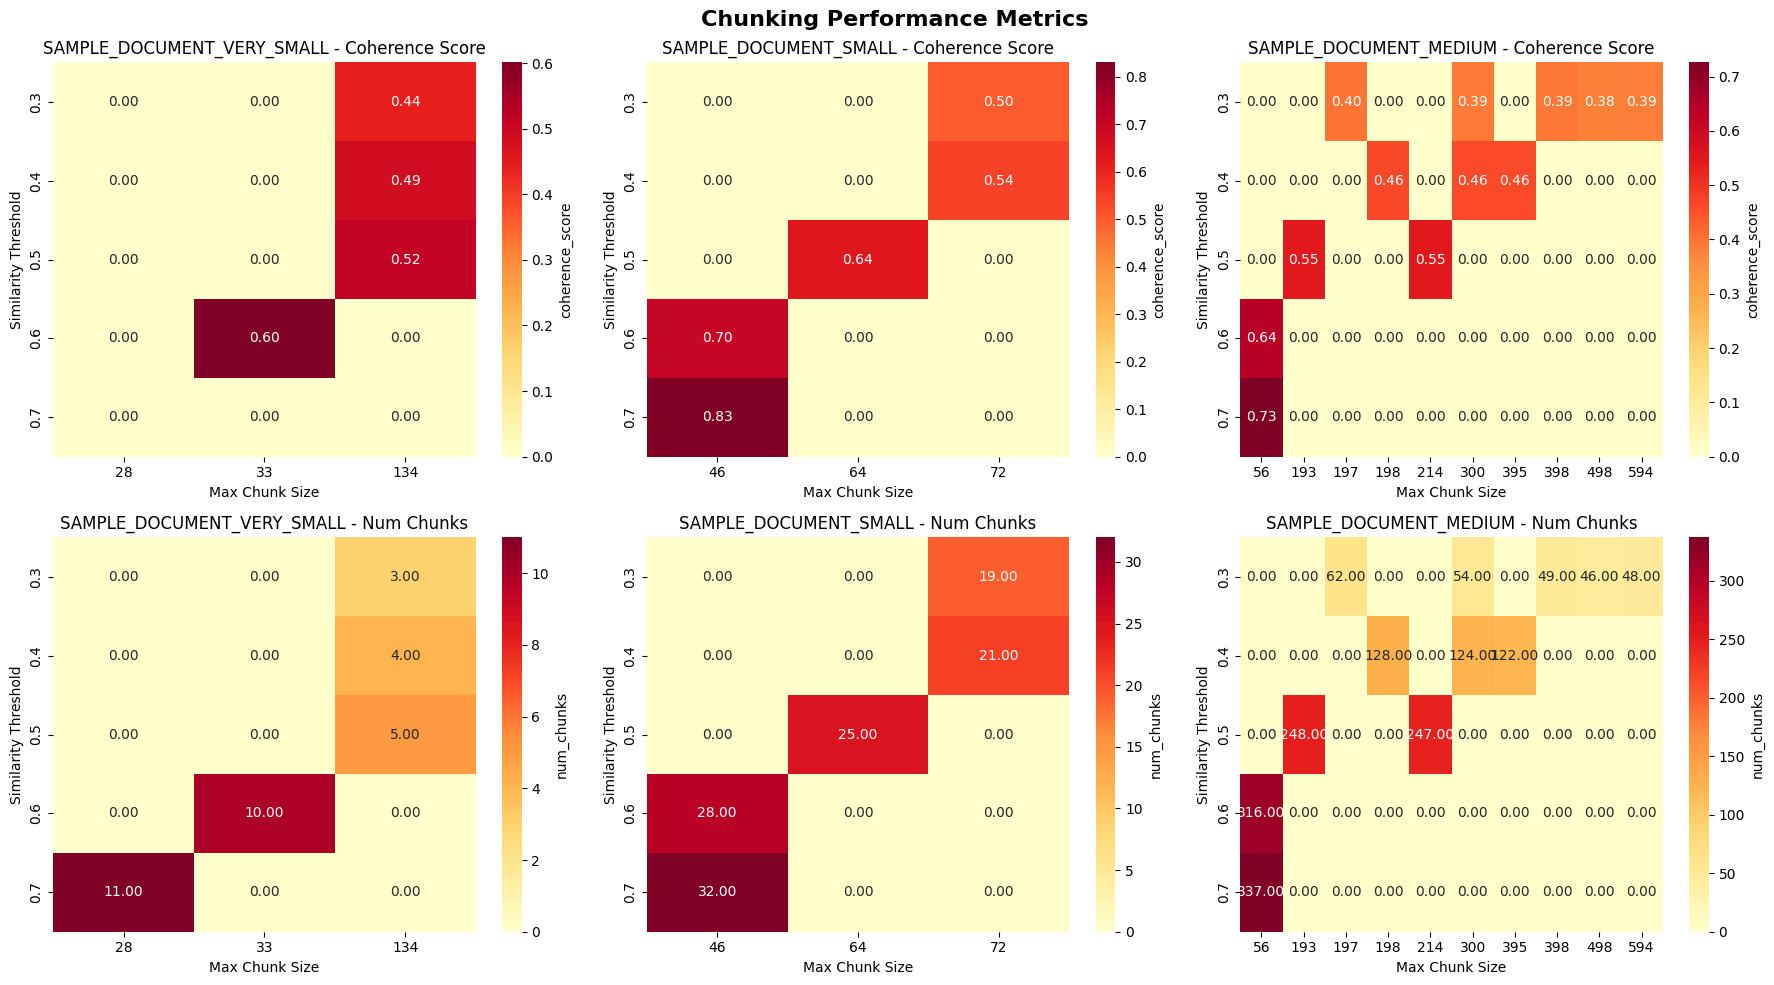
\includegraphics[width=0.8\textwidth]{assets/chunking_performance.png}
    \caption{Threshold and maximum chunking tests}
    \label{fig:chunk_thresholds}
\end{figure}

\paragraph{Embedding Model Selection}

The system uses the \textbf{all-MiniLM-L6-v2} embedding model, selected due to its performance–efficiency tradeoff and suitability for local execution. Its main characteristics are:

\begin{itemize}
    \item \textbf{Model size:} 22.7M parameters ($\sim$80 MB)
    \item \textbf{Embedding dimensionality:} 384
    \item \textbf{Training data:} Approximately 1 billion sentence pairs, including datasets such as Reddit (2015–2018), S2ORC citation pairs, and WikiAnswers.
    \item \textbf{Execution environment:} Fully local, ensuring privacy and avoiding vendor lock-in.
\end{itemize}

This model provides robust semantic discrimination while maintaining fast inference times, making it ideal for compliance workflows involving frequent document updates.

\paragraph{Reasoner: LLM-Based Compliance Engine}

To evaluate compliance between code snippets and document rules, the system uses the \textbf{Llama 3.1-70B Instruct} model hosted on the Hugging Face Inference API. The model performs the following tasks:

\begin{itemize}
    \item Interpreting rules extracted from the uploaded document.
    \item Comparing them to a given code sample.
    \item Identifying violations or missing implementations.
    \item Generating human-readable explanations and potential remediation steps.
\end{itemize}

\textbf{Model specifications:}
\begin{itemize}
    \item \textbf{Parameters:} 70 billion
    \item \textbf{Training data:} Instruction datasets from books, academic corpora, technical specifications, and over 25 million synthetic examples.
    \item \textbf{Output format:} A structured JSON object for programmatic consumption.
\end{itemize}

\subparagraph{Example Output}

\begin{verbatim}
{
  "compliant": false,
  "violations": [
    { "rule": "...", "description": "...", "fix": "..." }
  ],
  "missing_implementations": [],
  "summary": "..."
}
\end{verbatim}

\section{Pull Request Agent}

The Pull Request Agent is a specialized component designed to automate the code review process for external contributions hosted on version control platforms (e.g., GitHub). Unlike the standard Review Agent, which focuses on refining local files for readability, the Pull Request Agent acts as a strict Senior Software Engineer, analyzing specific code changes (diffs) and providing feedback directly on the pull request.

Key responsibilities include:

\begin{itemize}
    \item \textbf{Diff-Based Analysis:} The agent fetches the raw patch data from a pull request and parses it to identify added or modified lines. It strictly targets its analysis to these changes to ensure relevance.
    \item \textbf{Critical Validation:} It evaluates code for potential bugs, security vulnerabilities, naming conventions, and optimization opportunities.
    \item \textbf{Noise Reduction:} To prevent overwhelming developers, the agent is configured to prioritize the most significant issues, limiting its output to a maximum of two comments per file.
    \item \textbf{GitHub Integration:} Instead of modifying local files, this agent interfaces with the GitHub API to post line-specific review comments directly onto the pull request timeline.
\end{itemize}

\paragraph{Communication Behavior}

\begin{figure}[h!]
    \centering
    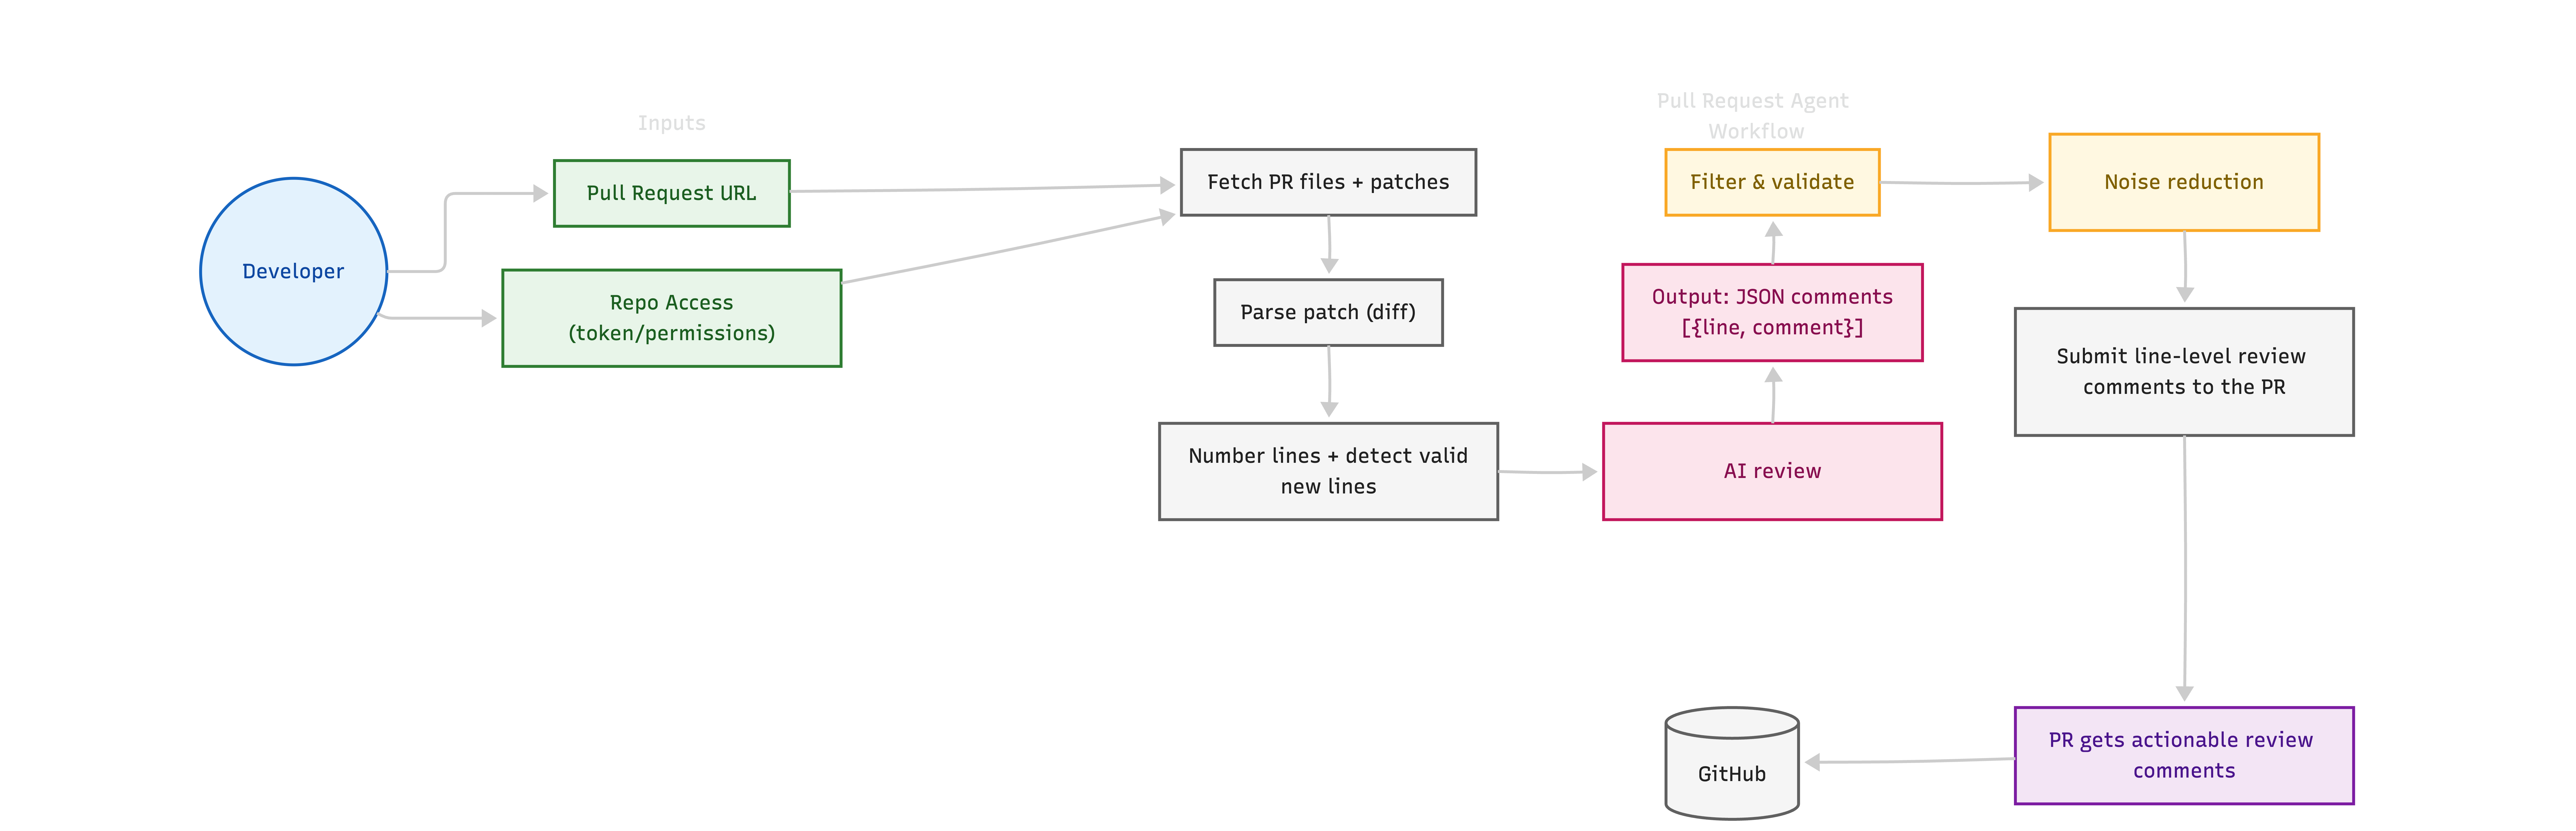
\includegraphics[width=1\textwidth]{assets/PR_diagram.png}
    \caption{Pull request agent's workflow}
    \label{fig:design}
\end{figure}

The Pull Request Agent follows a distinct workflow separate from the primary development pipeline:
\[
\textbf{Fetch PR} \rightarrow \textbf{Parse Patch} \rightarrow \textbf{AI Analysis} \rightarrow \textbf{Filter \& Submit}
\]

It accepts a filename and numbered diff content as input and outputs a structured JSON object containing a list of review comments:

\begin{verbatim}
{
  "reviews": [
    { 
      "line": 42, 
      "comment": "Potential security risk: input is not validated." 
    }
  ]
}
\end{verbatim}

The system implements a robust filtering mechanism that cross-references AI-generated line numbers with the actual patch data, discarding any comments that reference unchanged or invalid lines before submission.
\section{Security Agent: Real-Time Line Validator}

The system incorporates a specialized security component, the \texttt{LineValidator}, which operates within the Visual Studio Code environment to provide immediate feedback on code safety as it is being written. 

\begin{figure}[h!]
    \centering
    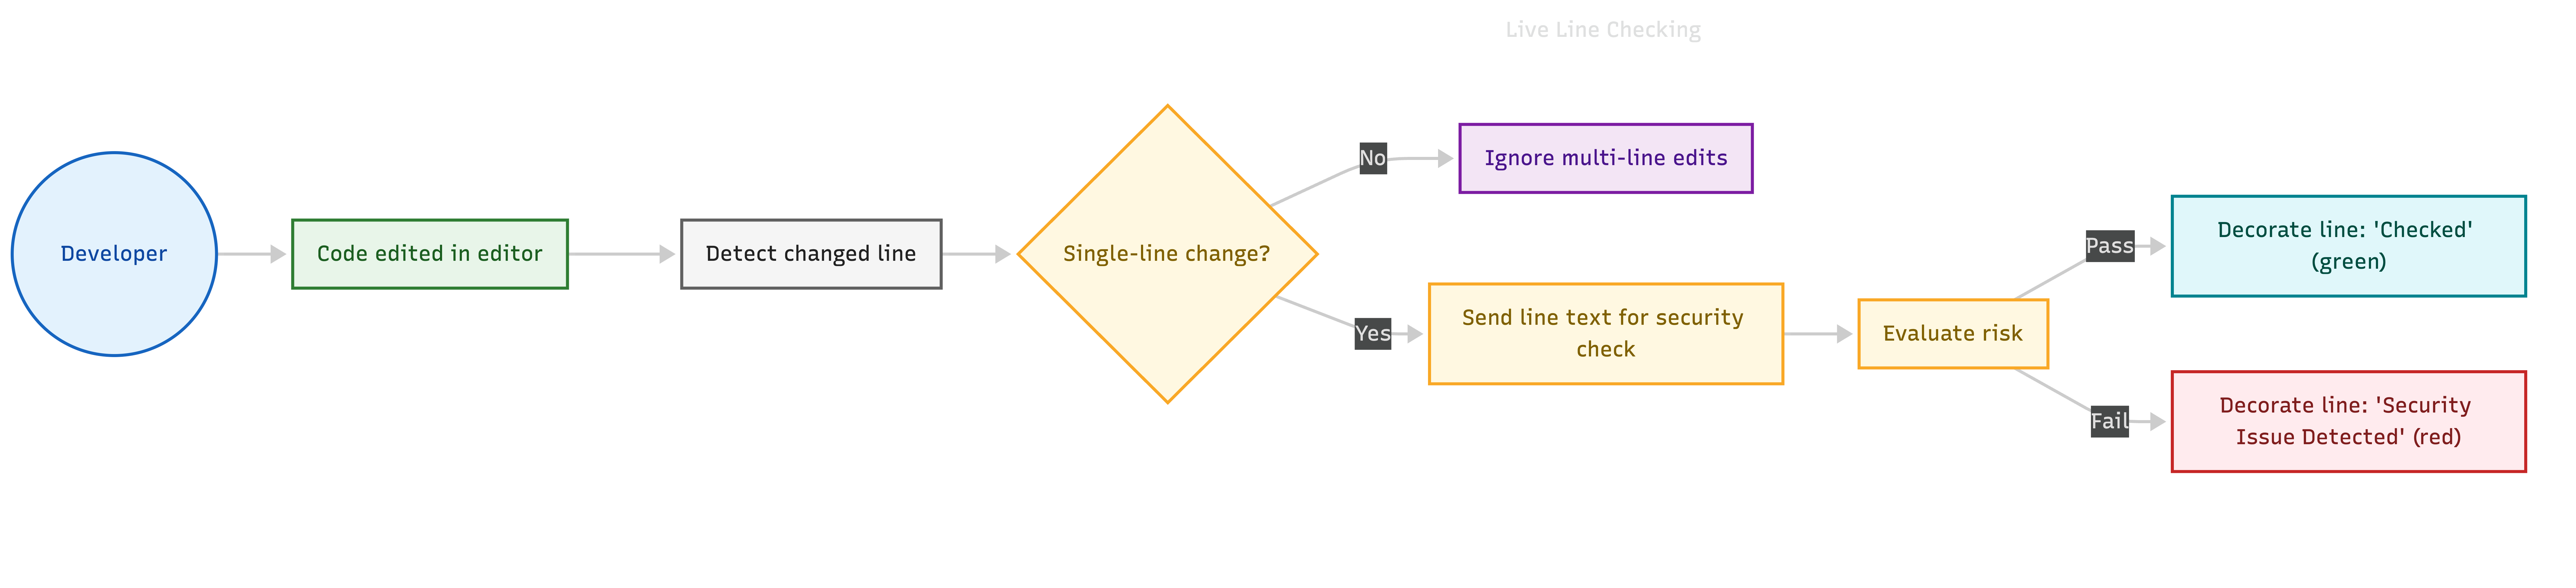
\includegraphics[width=1\textwidth]{assets/S_diagram.png}
    \caption{Workflow diagram for Security Agent}
    \label{fig:design}
\end{figure}

\subsection{Operational Mechanism}

The Security Agent monitors the \texttt{onDidChangeTextDocument} event in the editor. It triggers a validation check specifically when a user presses the \textit{Enter} key, signaling the completion of a line. To minimize noise, the agent only processes lines that contain at least four characters.

\subsection{Visual Feedback and Intent}

Once a line is validated, the agent applies temporary text decorations directly in the editor to inform the developer of the result:
\begin{itemize}
    \item \textbf{Checked (Green):} Indicates the line has been scanned and no immediate issues were found.
    \item \textbf{Security Issue Detected (Red):} Alerts the user to a potential vulnerability or bad practice detected in that specific line.
\end{itemize}

These decorations are designed to be non-intrusive, automatically disappearing after a 1.5-second timeout to maintain a clean workspace.
\section{Agent Evaluation: The Judge System}

To ensure the reliability and continuous improvement of the multi-agent orchestration, the project includes an automated evaluation framework called the \texttt{Judge}. This system acts as an independent auditor that analyzes the execution logs of all agents in the pipeline.

\subsection{Evaluation Criteria}

The Judge utilizes the \texttt{gpt-4o-mini} model to review each step of an agent's execution based on a structured prompt. It evaluates the \textit{Main}, \textit{Architecture}, \textit{Builder}, and \textit{Reviewer} agents, producing a standardized JSON report for every step with the following attributes:
\begin{itemize}
    \item \textbf{Grade:} An integer from 0 to 10 reflecting the quality and success of the agent's action.
    \item \textbf{Observations:} A concise summary identifying what went well or where the agent failed.
    \item \textbf{Future Context:} Key knowledge points that must be passed to the subsequent execution step to maintain coherence.
\end{itemize}

\subsection{Performance Visualization}

The system processes raw log files from the server's \texttt{runs/} directory and aggregates the scores into a persistent history. It automatically generates a performance plot for each run, allowing developers to visually track agent efficiency across complex multi-step tasks.

\begin{figure}[h!]
    \centering
    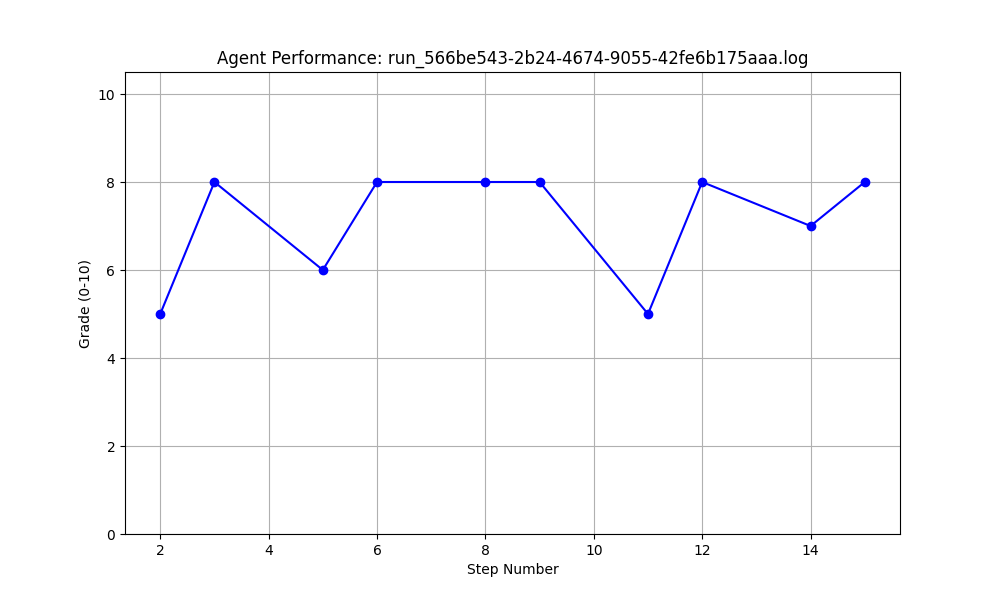
\includegraphics[width=1\textwidth]{assets/grades_plot.png}
    \caption{Example performance plot}
    \label{fig:design}
\end{figure}

\newpage
\section{Implementation Details}

This section presents the concrete implementation work carried out during the development of the 
Visual Studio Code extension.

\begin{figure}[h!]
    \centering
    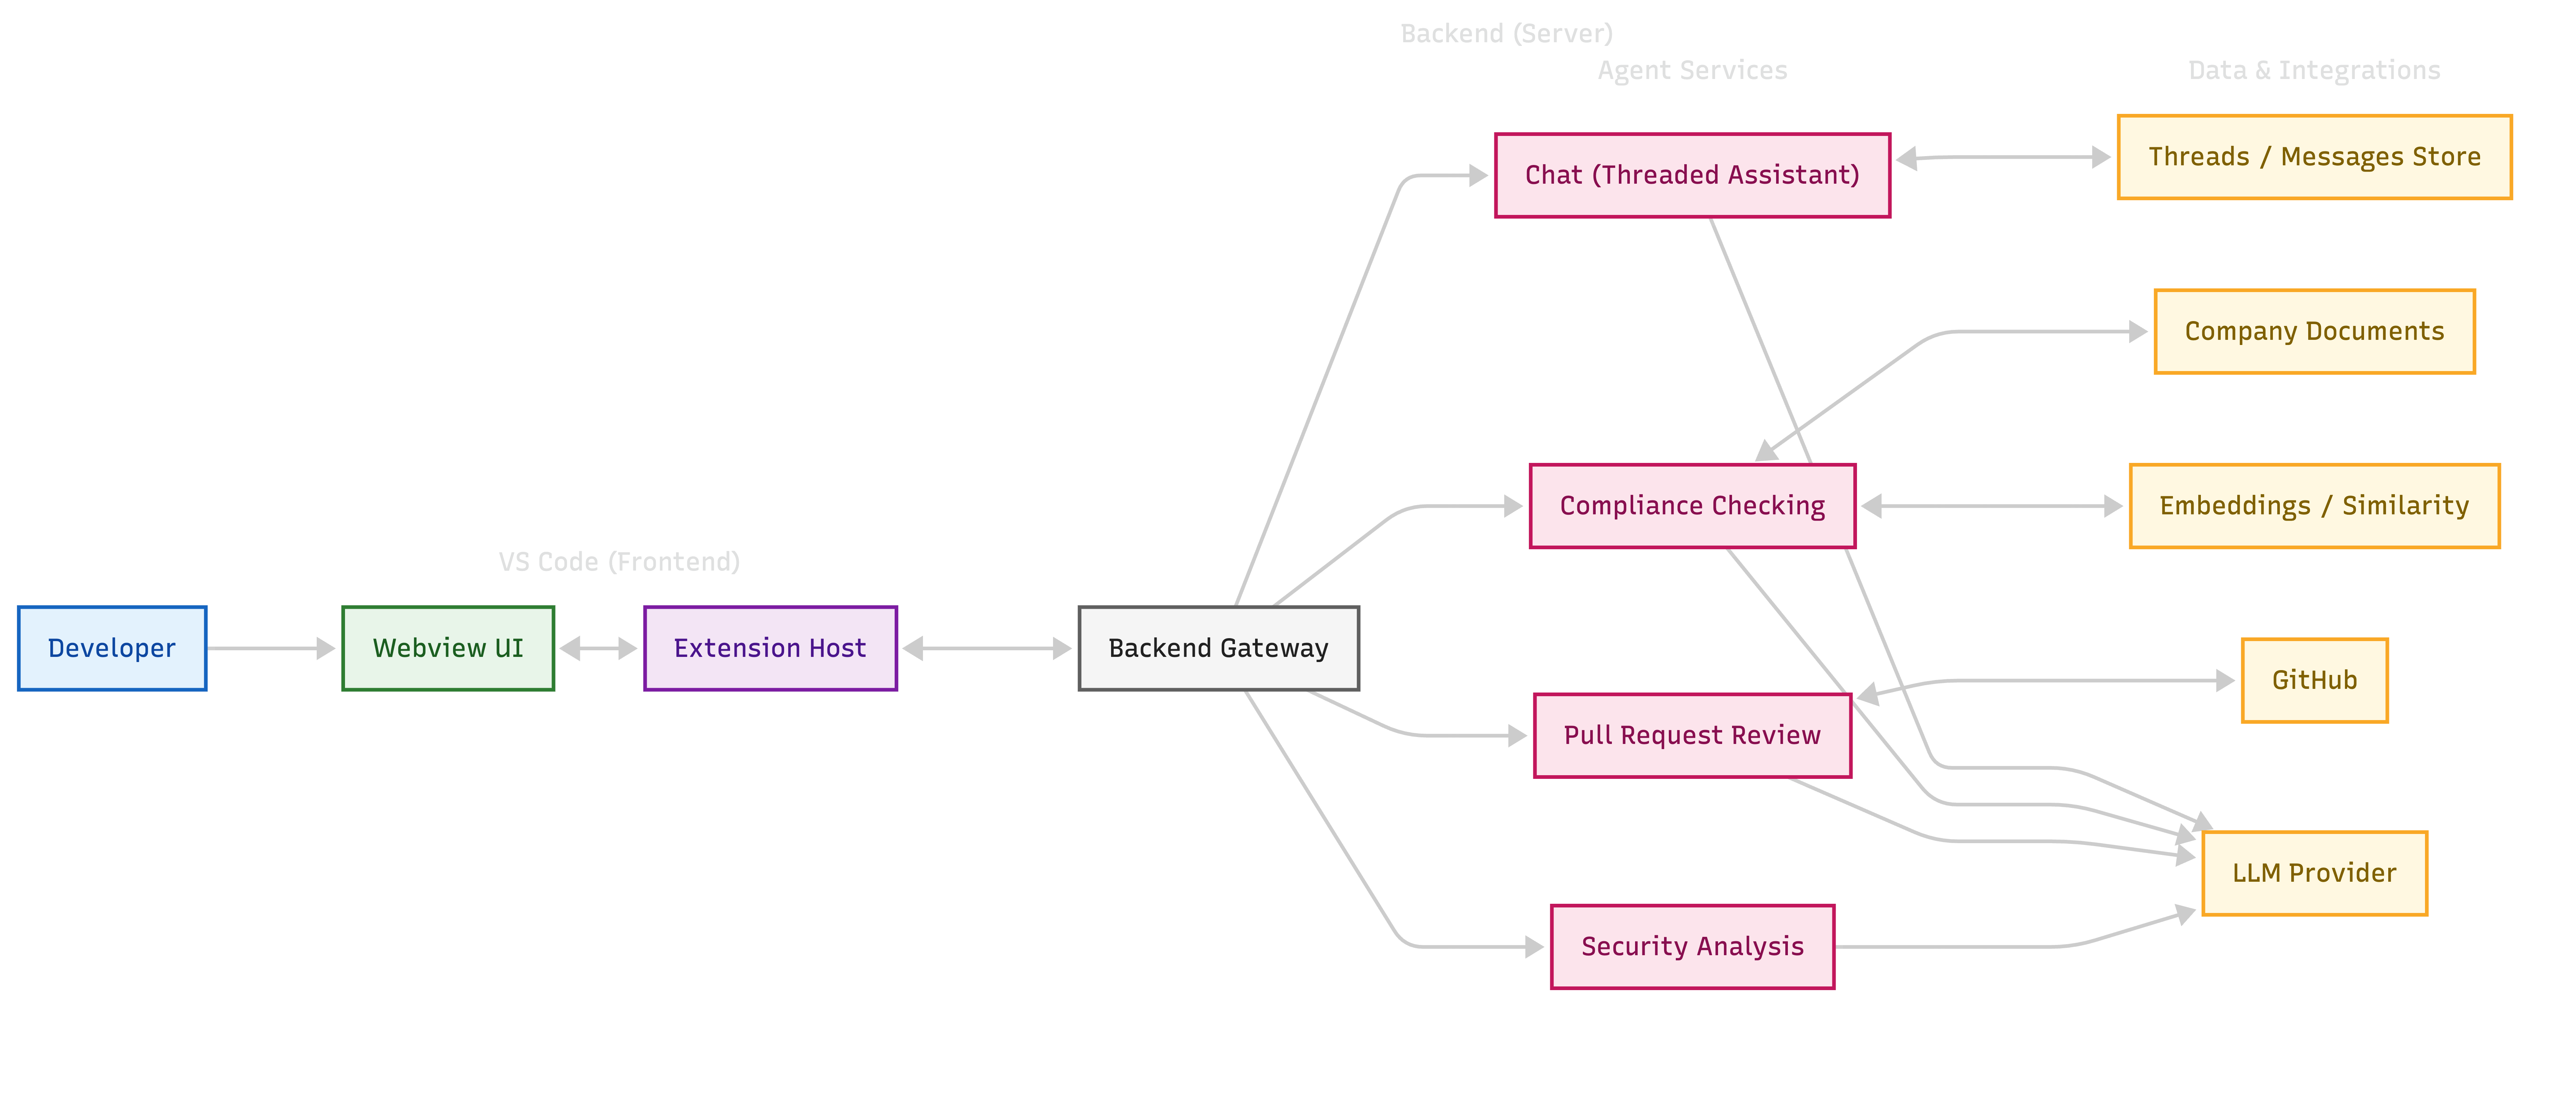
\includegraphics[width=1\textwidth]{assets/Sys_Arch_diagram.png}
    \caption{Application architecture}
    \label{fig:design}
\end{figure}

\subsection{Backend Architecture and Persistence}

The server-side implementation is built on Django and provides a scalable foundation for multi-agent interactions.
\begin{itemize}
    \item \textbf{Data Modeling:} The system tracks conversation history through the \texttt{Thread} and \texttt{Message} models. Each message records the specific agent involved and the number of tokens consumed for that interaction.
    \item \textbf{Orchestration Service:} The \texttt{ChatbotService} manages the core execution loop. It handles agent transitions by interpreting the \texttt{target} field in the AI's response, determining whether to call the next agent or return a result to the user.
    \item \textbf{REST API:} Frontend communication is facilitated through specialized views that handle message sending, long-polling for thread updates, and project file uploads.
\end{itemize}

\subsection{VS Code Extension Integration}

The client-side extension is integrated into VS Code using TypeScript and the Webview API.
\begin{itemize}
    \item \textbf{Chat Sidebar:} The extension registers a \texttt{WebviewViewProvider} to render a persistent chat interface within the sidebar.
    \item \textbf{Workspace Commands:} It registers commands such as \texttt{extension.analyzeProject} which allows users to trigger a manual scan of the directory structure.
    \item \textbf{Output Channels:} A dedicated \texttt{ANALYSIS\_CHANNEL} is used to stream real-time logs and project analysis results to the user, ensuring transparency in the assistant's reasoning process.
\end{itemize}

\subsection{Communication Model}

The communication between the frontend and the backend is implemented using a message–based protocol based on the Visual Studio Code \texttt{vscode.postMessage} API and a persistent backend service built in Node.js. The architecture follows a bidirectional message flow:

\begin{itemize}
    \item \textbf{Frontend → Backend:} User messages, file queries, command triggers, and agent delegation requests.
    \item \textbf{Backend → Frontend:} Agent responses, updated generation states, progress indicators, final code outputs, and error events.
\end{itemize}

This design ensures a non-blocking, event-driven pipeline suitable for long-running tasks such as code generation, multi-step reasoning, or incremental file retrieval.

\subsection{File Retrieval System}
One of the key technical contributions is the implementation of a robust file-retrieval mechanism 
enabling the Main Agent to request the project’s workspace tree only when needed. This provides the 
AI system with contextual knowledge while preserving memory efficiency and token budget constraints. 
\newline

Before the introduction of the \texttt{getFile} system, the Main Agent was unaware of the project’s 
directory structure unless the entire tree was preloaded. This posed several problems:

\begin{itemize}
    \item unnecessary token consumption for large projects,
    \item unnecessary delays caused by loading unused directories,
    \item inability of the Main Agent to dynamically request missing context,
    \item higher risk of hallucinations when referencing files not yet retrieved.
\end{itemize}

The new approach introduces a demand-driven information flow where file context is requested only 
when explicitly required by the agent pipeline. The file tree is returned using the previously 
described \textbf{TOON (Token-Oriented Object Notation)} format. The integration of TOON into the 
file retrieval mechanism results in several benefits:

\begin{itemize}
    \item \textbf{Reduced token overhead} compared to JSON-based structures.
    \item \textbf{Improved LLM interpretability} due to indentation hierarchy.
    \item \textbf{Adaptive delimiter usage} for filenames containing special characters.
    \item \textbf{Explicit element counts} improving structural robustness.
\end{itemize}
\end{document}